\documentclass[12pt,titlepage] {article}
\usepackage[utf8] {inputenc}
\usepackage[finnish] {babel}
\usepackage {amsmath}
\usepackage {amssymb}
\usepackage {amsthm}
\usepackage {mathtools}
\usepackage {graphicx}
\usepackage {listings}
\usepackage {xcolor}

\DeclarePairedDelimiter\floor{\lfloor}{\rfloor}

\lstset{basicstyle=\ttfamily\footnotesize, keywordstyle=\color{blue}, commentstyle=\color{green}, breaklines=true, numbers=left, frame=single, literate={ö}{{\"o}}1{ä}{{\"a}}1}

\begin {document}

\title {Tietokannat - harjoitustyö (osa 1)}
\author {Miska Kananen (652102, miska.kananen@aalto.fi) \\ Teemu Mäkinen (628835, teemu.v.makinen@aalto.fi)}
\date {\today}
\maketitle

\section {UML-kaavio}

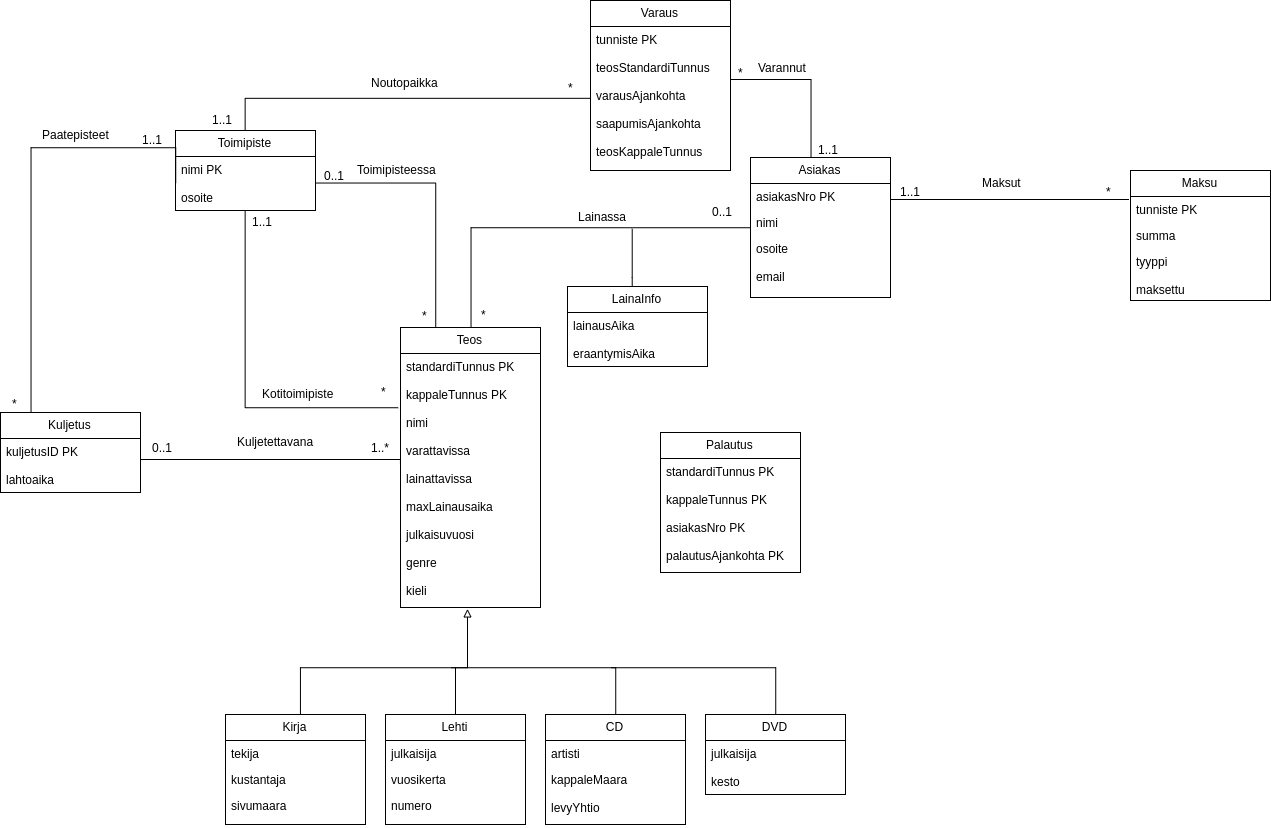
\includegraphics[width=\textwidth]{kirjasto.png}

\section {Relaatiokaavio}

\begin{itemize}
	\item \texttt{Teos(\underline{standardiTunnus}, \underline{kappaleTunnus}, nimi, varattavissa, lainattavissa, maxLainausaika, julkaisuvuosi, genre, kieli)}
	\item \texttt{Kirja(\underline{standardiTunnus}, \underline{kappaleTunnus}, tekija, kustantaja, sivumaara)}
	\item \texttt{Lehti(\underline{standardiTunnus}, \underline{kappaleTunnus}, julkaisija, vuosikerta, numero)}
	\item \texttt{CD(\underline{standardiTunnus}, \underline{kappaleTunnus}, artisti, kappaleMaara, levyYhtio)}
	\item \texttt{DVD(\underline{standardiTunnus}, \underline{kappaleTunnus}, julkaisija, kesto)}
	\item \texttt{Asiakas(\underline{asiakasNro}, nimi, osoite, email)}
	\item \texttt{Varaus(\underline{tunniste}, teosStandardiTunnus, varausAjankohta, saapumisAjankohta, teosKappaleTunnus)}
	\item \texttt{Palautus(\underline{standardiTunnus}, \underline{kappaleTunnus}, \underline{asiakasNro}, \underline{palautusAjankohta})}
	\item \texttt{Maksu(\underline{tunniste}, summa, tyyppi, maksettu)}
	\item \texttt{Toimipiste(\underline{nimi}, osoite)}
	\item \texttt{Kuljetus(\underline{kuljetusID}, lahtoaika)}
\end{itemize}

\begin{itemize}
	\item \texttt{Lainassa(\underline{standardiTunnus}, \underline{kappaleTunnus}, asiakasNro, lainausAika, eraantymisAika)}
	\item \texttt{Maksut(\underline{maksuTunniste}, asiakasNro)}
	\item \texttt{Varannut(\underline{varausTunniste}, asiakasNro)}
	\item \texttt{Noutopaikka(\underline{varausTunniste}, toimipisteNimi)}
	\item \texttt{Toimipisteessa(\underline{standardiTunnus}, \underline{kappaleTunnus}, toimipisteNimi)}
	\item \texttt{Kotitoimipiste(\underline{standardiTunnus}, \underline{kappaleTunnus}, toimipisteNimi)}
	\item \texttt{Paatepisteet(\underline{kuljetusID}, lahtoToimipiste, paateToimipiste)}
	\item \texttt{Kuljetettavana(\underline{standardiTunnus}, \underline{kappaleTunnus}, kuljetusID)}
\end{itemize}

\section {Selostus ratkaisusta}

Kirjaston teoksia kuvataan \texttt{Teos}-relaatiolla, jonka yksi monikko kuvaa tietyn teoksen yksittäistä kappaletta. Relaation avain koostuu standarditunnuksesta, joka yksilöi teoksen ja kappaletunnuksesta, joka yksilöi yksittäisen kappaleen tietystä teoksesta. Standarditunnus on esim. kirjoilla ISBN ja lehdillä ISSN. Kappaletunnuksena voi toimia esimerkiksi juokseva numerointi. Yksittäiselle kappaleelle voi määrittää sen attribuutteina, onko se varattavissa ja lainattavissa ja jos on, kuinka pitkäksi aikaa.

\texttt{Teos}-relaatio sisältää kaikille teoksille yhteiset ominaisuudet, kuten kieli ja genre, ja teostyypeille spesifit ominaisuudet on määritelty \texttt{Kirja}, \texttt{Lehti}, \texttt{CD} ja \texttt{DVD} -relaatioissa. Kaikki teokset ovat joko kirjoja, lehtiä, CD:itä tai DVD:itä.

Yksittäinen teoksen kappale on kulloinkin joko jossakin toimipisteessä, lainassa tai kuljetettavana. Relaatiot \texttt{Toimipisteessa}, \texttt{Lainassa} ja \texttt{Kuljetettavana} kertovat, mitä teoksia on kulloinkin kyseisissä paikoissa. Kun kappaleen paikka muuttuu esimerkiksi lainauksen tai kuljetuksen yhteydessä, päivitetään relaatioita vastaavasti.

Kirjaston asiakkaita kuvataan \texttt{Asiakas}-relaatiolla, ja yksittäinen asiakas yksilöidään asiakasnumerolla, joka voi olla esimerkiksi juokseva numerointi. Asiakkaista tallennetaan oleelliset henkilötiedot, kuten nimi ja osoite.

Asiakkaiden maksettavia maksuja kuvataan \texttt{Maksu}-relaatiolla. Kullakin maksulla on yksiselitteinen tunniste, joka voi olla esim. juokseva numerointi, summa, tyyppi, kuten varausmaksu tai myöhästymismaksu ja tieto siitä, onko asiakas maksanut maksun.

Relaatio \texttt{Varaus} kuvaa tiettyyn teokseen kohdistuvaa varausta. Varaukseen tallennetaan teoksen standarditunnus, joka määrittää, mihin teokseen varaus kohdistuu, sekä varausajankohta, joka määrittää varauksen sijainnin varausjonossa. 

Niin kauan kuin asiakkaalle ei ole tarjottu varausta noudettavaksi, varaus kohdistuu kaikkiin teoksen kappaleisiin ja mitään yksittäistä kappaletunnusta ei ole määritelty. Kun jokin teoksen kappale vapautuu, kohdistetaan varaus kyseiseen kappaleeseen, eikä varaus enää vaikuta teoksen muihin kappaleisiin. 

Saapumisajankohta kertoo, onko varauksen teos saapunut noudettavaksi, ja jos on, milloin. Sen perusteella määritetään, milloin asiakkaan on viimeistään noudettava varaus. Jos varausta ei noudeta ajoissa, se siirtyy seuraavan jonottajan noudettavaksi, tai jos varauksia ei enää ole, vapautuu vapaasti lainattavaksi ja palautuu tarvittaessa kotitoimipisteeseen.

Teoksien kappaleita voidaan joutua kuljettamaan toimipisteiden välillä, jos kappale palautetaan muualle kuin sen kotitoimipisteeseen, tai jos kappale varataan noudettavaksi jostakin muusta toimipisteestä. Kuljetuksia kahden toimipisteen välillä kuvataan \texttt{Kuljetus}-relaatiolla, jonka monikko vastaa yksittäistä kuljetusta. Kuljetuksella on yksiselitteinen tunniste, joka voi olla esimerkiksi juokseva numerointi, ja lähtöaika.

Jos jokin kappale pitää kuljettaa toiseen toimipisteeseen, voidaan \texttt{Kuljetus}-relaatiosta selvittää, onko jo olemassa sopivaa kuljetusta, joka ei ole lähtenyt vielä. Tällöin kappale voidaan laittaa kyseisen kuljetuksen kyytiin, muussa tapauksessa järjestetään uusi kuljetus.

Kun asiakas lainaa teoksen kappaleen, se lisätään \texttt{Lainassa}-relaatioon ja poistetaan \texttt{Toimipisteessa}-relaatiosta. Relaatioon tallennetaan lainauspäivämäärä ja lainan erääntymispäivämäärä, joka voidaan määrittää esimerkiksi kappaleen maksimilainausajan perusteella.

Kun asiakas palauttaa teoksen, se poistetaan \texttt{Lainassa}-relaatiosta ja lisätään asianmukaiseen \texttt{Toimipisteessa}-relaatioon. Palautustapahtumaa kuvaava monikko lisätään \texttt{Palautus}-relaatioon, joka toimii kirjaston palautuslokina.

Uusia toimipisteitä, asiakkaita, teoksia ja kappaleita voidaan lisätä yksinkertaisesti lisäämällä vastaaviin relaatioihin uusi monikko.

Ne toimipisteet, joissa on vapaana teoksen kappale, voidaan selvittää etsimällä kullekin toimipisteelle \texttt{Toimipisteessa}-relaatiosta teoksen standarditunnusta vastaavat monikot ja ottamalla \texttt{Teos}-relaatiosta niitä vastaavat monikot, jotka kuvaavat toimipisteessä olevia kappaleita. Kappaleissa voi olla kuitenkin vielä varauksia, joten poistetaan monikoista ne kappaleet, joiden standarditunnus ja kappaletunnus esiintyy jossakin \texttt{Varaus}-relaation monikossa.

Käyttäjällä lainassa olevat teokset ja niiden erääntymispäivät voi kysyä suoraan \texttt{Lainassa}-relaatiosta.

Tietyn kappaleen edelliset lainaajat voi selvittää \texttt{Palautus}-relaatiosta teoksen standarditunnuksen ja kappaletunnuksen perusteella järjestämällä monikot palautusajankohdan mukaan laskevaan järjestykseen ja ottamalla vastaavat asiakasnumerot.

Teoksia voidaan hakea erilaisten hakuehtojen mukaan kohdistamalla haun \texttt{Teos}-relaatioon sekä \texttt{Kirja}, \texttt{Lehti}, \texttt{CD} ja \texttt{DVD}-relaatioihin.

Kun teoksen kappale palautetaan johonkin toimipisteeseen, tarkistetaan ensin \texttt{Varaus}-relaatiosta, kohdistuuko teokseen varauksia. Jos kohdistuu, etsitään aikaisin varaus, joka odottaa kappaleen vapautumista eli jolle ei ole vielä määritelty kappaleen tunnusta, ja yhdistetään palautettu kappale varaukseen. Jos kappale on määritelty varauksessa noudettavaksi toisesta toimipisteestä, järjestetään kappaleelle kuljetus. Jos teokseen ei kohdistu varauksia, mutta se on väärässä toimipisteessä, kuljetetaan se takaisin kotitoimipisteeseen.

Myöhästyneet lainat voidaan selvittää \texttt{Lainassa}-relaatiosta etsimällä ne lainat, joiden erääntymisaika on mennyt. Teoksen lainannut asiakas saadaan selville samasta relaatiosta.

Asiakkaan maksamatta olevat maksut voi selvittää \texttt{Maksut}-relaatiosta etsimällä ne \texttt{Maksu}-relaation monikot, joita ei ole vielä merkitty maksetuiksi.

\section {Funktionaaliset riippuvuudet}

Teoksen standarditunnus yksilöi teoksen, ja kaikilla tietyn teoksen kappaleilla on samoja ominaisuuksia:

\begin{itemize}
\item Relaatiossa \texttt{Teos} $standardiTunnus \rightarrow nimi\ julkaisuvuosi\ kieli\ genre$.
\item Relaatiossa \texttt{Kirja} $standardiTunnus \rightarrow tekija\ kustantaja\ sivumaara$.
\item Relaatiossa \texttt{Lehti} $standardiTunnus \rightarrow julkaisija\ vuosikerta\ numero$.
\item Relaatiossa \texttt{CD} $standardiTunnus \rightarrow artisti\ kappaleMaara\ levyYhtio$.
\item Relaatiossa \texttt{DVD} $standardiTunnus \rightarrow julkaisija\ kesto$.
\end{itemize}

Lisäksi kaikissa relaatioissa avainattribuutit yhdessä määräävät muut attribuutit.

\section {Anomaliat}

Kun teoksen sijainti muuttuu, eli esimerkiksi teos lainataan, palautetaan tai kuljetetaan toiseen toimipisteeseen, pitää huolehtia, että relaatiot \texttt{Toimipisteessa}, \texttt{Lainassa}, \texttt{Kuljetettavana} ja \texttt{Varaus} pysyvät ajan tasalla.

Jos toimipisteen nimi vaihtuu, joudutaan päivittämään myös relaatiot \texttt{Paatepisteet, Kuljetettavana, Kotitoimipiste, Sijaitsee} ja \texttt{Noutopaikka}.

\section {Boyce-Codd -normaalimuoto}

Tietokanta on Boyce-Codd -normaalimuodossa lukuunottamatta relaatioita \texttt{Teos, Kirja, Lehti, CD} ja \texttt{DVD}. Ositetaan nämä relaatiot.

Relaatiossa \texttt{Teos(\underline{standardiTunnus}, \underline{kappaleTunnus}, nimi, varattavissa, lainattavissa, maxLainausaika, julkaisuvuosi, genre, kieli)} on voimassa riippuvuus $standardiTunnus \rightarrow nimi\ julkaisuvuosi\ genre\ kieli$, mutta $\{standardiTunnus\}^+ = \{standardiTunnus, nimi, julkaisuvuosi, genre, kieli\}$.

Ositetaan relaatio. Relaatioon \texttt{Teos2} tulee $\{standardiTunnus\}^+$:n attribuutit ja relaatioon \texttt{Teos3} tulee $standardiTunnus$ ja relaation \texttt{Teos} loput attribuutit.

Relaatiot ovat siis \texttt{Teos2(\underline{standardiTunnus}, nimi, julkaisuvuosi, genre, kieli)} ja \texttt{Teos3(\underline{standardiTunnus}, \underline{kappaleTunnus}, varattavissa, lainattavissa, maxLainausAika)}.

\texttt{Teos2}:ssa on voimassa vain riippuvuus $standardiTunnus \rightarrow nimi\ julkaisuvuosi\ genre\ kieli$, ja $\{Teos2\}^+ = \{standardiTunnus, nimi, julkaisuvuosi, genre, kieli\}$, joten \texttt{Teos2} on BCNF:ssä. 

\texttt{Teos3}:ssa on voimassa vain riippuvuus $standardiTunnus\ kappaleTunnus \rightarrow varattavissa\ lainattavissa\ maxLainausAika$, ja $\{standardiTunnus, kappaleTunnus\}^+ = \{standardiTunnus, kappaleTunnus, varattavissa, lainattavissa, maxLainausAika\}$, joten \texttt{Teos3} on BCNF:ssä.

Täysin vastaavalla päättelyllä voidaan osittaa relaatiot \texttt{Kirja}, \texttt{Lehti}, \texttt{CD} ja \texttt{DVD} aiemmin mainittujen funktionaalisten riippuvuuksien perusteella.

Relaation \texttt{Kirja(\underline{standardiTunnus}, \underline{kappaleTunnus}, tekija, kustantaja, sivumaara)} ositus BCNF:ään on \texttt{Kirja2(\underline{standardiTunnus}, tekija, kustantaja, sivumaara)} ja \texttt{Kirja3(\underline{standardiTunnus}, \underline{kappaleTunnus})}.

Relaation \texttt{Lehti(\underline{standardiTunnus}, \underline{kappaleTunnus}, julkaisija, vuosikerta, numero)} ositus BCNF:ään on \texttt{Lehti2(\underline{standardiTunnus}, julkaisija, vuosikerta, numero)} ja \texttt{Lehti3(\underline{standardiTunnus}, \underline{kappaleTunnus})}.

Relaation \texttt{CD(\underline{standardiTunnus}, \underline{kappaleTunnus}, artisti, kappaleMaara, levyYhtio)} ositus BCNF:ään on \texttt{CD2(\underline{standardiTunnus}, artisti, kappaleMaara, levyYhtio)} ja \texttt{CD3(\underline{standardiTunnus}, \underline{kappaleTunnus})}.

Relaation \texttt{DVD(\underline{standardiTunnus}, \underline{kappaleTunnus}, julkaisija, kesto)} ositus BCNF:ään on \texttt{DVD2(\underline{standardiTunnus}, julkaisija, kesto)} ja \texttt{DVD3(\underline{standardiTunnus}, \underline{kappaleTunnus})}.

\section {1. osan palautuksen jälkeen tehdyt muutokset}

\subsection {Relaatiokaavio}

Poistetaan tarpeettomia monesta yhteen -assosiaatioista muodostettuja relaatioita. Poistetaan relaatiot \texttt{Paatepisteet}, \texttt{Maksut}, \texttt{Varannut}, \texttt{Noutopaikka} ja \texttt{Kotitoimipiste} ja yhdistetään niiden tiedot vastaaviin monesta-puolen relaatioihin.

Muutetaan \texttt{Palautus}-relaation avainta: asiakasnumeron ei tarvitse olla avaimena, koska tietty teoksen kappale voidaan palauttaa vain kerran tiettynä ajanhetkenä.

Erotetaan teoksen yleiset ja kappalekohtaiset tiedot kahdeksi eri relaatioksi \texttt{Teos} ja \texttt{Kappale}. Relaatio on tällöin BCNF:ssä.

Poistetaan kappaletunnus relaatioista \texttt{Kirja}, \texttt{Lehti}, \texttt{CD} ja \texttt{DVD}. Tällöin relaatiot ovat BCNF:ssä.

Uusi relaatiokaavio on:

\begin{itemize}
	\item \texttt{Teos(\underline{standardiTunnus}, nimi, julkaisuvuosi, genre, kieli)}
	\item \texttt{Kappale(\underline{standardiTunnus}, \underline{kappaleTunnus}, varattavissa, lainattavissa, maxLainausaika, kotitoimipiste)}
	\item \texttt{Kirja(\underline{standardiTunnus}, tekija, kustantaja, sivumaara)}
	\item \texttt{Lehti(\underline{standardiTunnus}, julkaisija, vuosikerta, numero)}
	\item \texttt{CD(\underline{standardiTunnus}, artisti, kappaleMaara, levyYhtio)}
	\item \texttt{DVD(\underline{standardiTunnus}, julkaisija, kesto)}
	\item \texttt{Asiakas(\underline{asiakasNro}, nimi, osoite, email)}
	\item \texttt{Varaus(\underline{tunniste}, teosStandardiTunnus, teosKappaleTunnus, varausAjankohta, saapumisAjankohta, varaajaAsiakasNro, noutoToimipiste)}
	\item \texttt{Palautus(\underline{standardiTunnus}, \underline{kappaleTunnus}, \underline{palautusAjankohta}, asiakasNro)}
	\item \texttt{Maksu(\underline{tunniste}, summa, tyyppi, maksettu, asiakasNro)}
	\item \texttt{Toimipiste(\underline{nimi}, osoite)}
	\item \texttt{Kuljetus(\underline{kuljetusID}, lahtoaika, lahtoToimipiste, paateToimipiste)}
\end{itemize}

\begin{itemize}
	\item \texttt{Lainassa(\underline{standardiTunnus}, \underline{kappaleTunnus}, lainausAika, eraantymisAika, asiakasNro)}
	\item \texttt{Toimipisteessa(\underline{standardiTunnus}, \underline{kappaleTunnus}, toimipisteNimi)}
	\item \texttt{Kuljetettavana(\underline{standardiTunnus}, \underline{kappaleTunnus}, kuljetusID)}
\end{itemize}

\section {Tietokannan luominen}

\lstinputlisting[language=SQL]{create_tables.sql}

\section {Hakemistot ja näkymät}

\lstinputlisting[language=SQL]{hakemistot_nakymat.sql}

\section {Käyttötapaukset}

\lstinputlisting[language=SQL]{kayttotapaukset.sql}

\end {document}
